\section{Cooperative Controllers}


\subsection{Overview Cooperative Controllers}

Assistive controllers have long been implemented in rehabilitative exoskeletons. This includes the MIT-MANUS \cite{ju2005rehabilitation}, BLEEX\cite{kazerooni2006hybrid}, HAL\cite{kawamoto2004power} and many others robotic systems including several exoskeletons \cite{kim2012admittance,ott2010unified,huo2011control}. These systems use assistive controllers to help guide the person's arm or leg through some desired trajectory or complete tasks. This method is typically used because the person has difficulty generating the necessary torques due to medical problems such as a stroke or spinal cord injury. The difficulty in designing these systems is in handling the non-linearity and distances from being connected to a person, which the controller will have to overcome. Many of these controllers implement either impedance or admittance models. Admittance controllers transform forces and torques to the desired position and orientation. Impedance controllers are the mirror calculating displacements from applied forces and torques. They allow for virtual stiffness, which is useful for controlling the human-robot interactions \cite{keemink2018admittance}. 

The admittance controller has shown better results when implemented into an exoskeleton. They are easier to implement and can measure the intention of the user. Admittance controllers allow for the adjustment of the stiffness to meet the on-the-fly demand by either being more or less aggressive in the supplied force \cite{aguirre2007active,newman1994stable}. This problem is solved by using variable admittance, where the parameters are adjusted based on the user's intention and ability.

Oh \textit{et. al} proposed a generalized framework for assistive controllers \cite{oh2015generalized}. The proposed controller combined a model-based method with feed-forward disturbance rejection—this method models the interaction as a disturbance to the system instead of an interactive force.  Additionally, a PD controller was used, in contrast to a Sliding Mode Controller (SMC), which has been shown to have better performance in controlling non-linear systems. They both have robust and adaptive properties that are ideal for assistive systems \cite{slotine1991applied}.

SMC is a popular method in assistive controllers due to their insensitivity to disturbances and handling of non-linearity better than traditional PD controller \cite{nasir2010performance} \cite{sanngoen2020review} \cite{fischer-SMC}. SMC works by using a switching function to drive the system along a sliding surface. Torabi \textit{et al.} used a model-based SMC controller to drive a lower limb exoskeleton. This controller also used an adaptive admittance controller along with the SMC to adjust to the user intention ability \cite{torabi2018robust}. A similar method of model-based SMC was used by Babaiasl \textit{et. al} to control an upper limb exoskeleton \cite{babaiasl2015sliding}. In \cite{long2016robust} a genetic algorithm was used to tune the parameters of an SMC for a lower limb exoskeleton. The parameters were tuned in MATLAB/SIMULINK. While successful, they did not model a connection between the human and exoskeleton and did not use an adaptive admittance controller. 

\begin{figure}
    \centering
    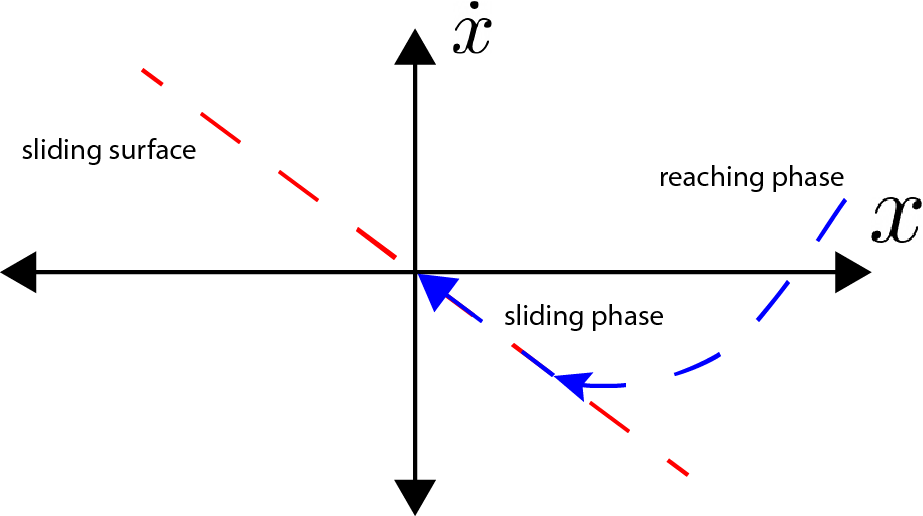
\includegraphics{images/controllers/SMC.png}
    \caption{Sliding mode control and the switching phase}
    \label{fig:SMC}
\end{figure}

\subsection{Development of Cooperative Controller and Tuning Methods}

In this section a method of developing a closed loop assastive controller will be discussed. First a simplified system is presented so that the controller can be developed. The simplified system constitutes of two double pendulums connected by a mass-spring dampener at each link. Then a method of tuning the parameters is presented along with the effects on effort reduction and system misalignment.

\autoref{fig:double_pend} illustrates the simplified system. Because one set of pendulums is being assisted by the other set, one pendulum is the \textit{assistie} and the other pendulum is the \textit{assisitor} system. The \textit{assisitor} system provides additional torques to help the \textit{assistie} to move through some desired motion. This model and controller are based on the work by Tu \textit{et. al} \cite{tu2020adaptive}, however the system was modified so that \textit{assistie} system is driven by a closed-loop controller. These changes add complexity to the system since the \textit{assistor} system has to handle the errors that arise in the attached closed-loop controller. With two closed-loop systems connected, the controller commands are magnified when handling the errors \cite{tu2020adaptive}. \autoref{fig:controlDiagram} shows the control diagram. The first model has a pendulum that is controlled by a simple closed-loop PD controller. The second model is controlled by an Admittance-Sliding Mode Controller (A-SMC), which has useful properties for handling non-linear dynamics and disturbances. Additionally, a gradient descent method is used to auto-tune the PD controller parameters and the A-SMC. 

The problem with A-SMC controllers is the large number of parameters that need to be tuned. These parameters can have non-linear and hard-to-determine effects on the response of the system \cite{slotine1983tracking}. These parameters include SMC parameters and the variable admittance model parameters. Both of which scale with the dimensions of the system. Having a comprehensive method to determine these parameters allows the system to be tuned automatically.  

\begin{figure}
    \centering
    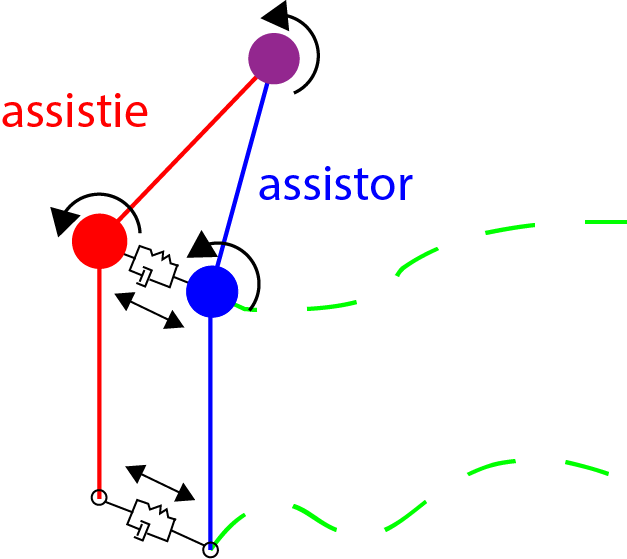
\includegraphics[scale=1.5]{images/controllers/double_pend.png}
    \caption{Double connected pendulum. Spring-dampeners connect the two pendulum (\textit{assistor} and \textit{assistie}) }
    \label{fig:double_pend}
\end{figure}

\begin{figure*}
    \centering
    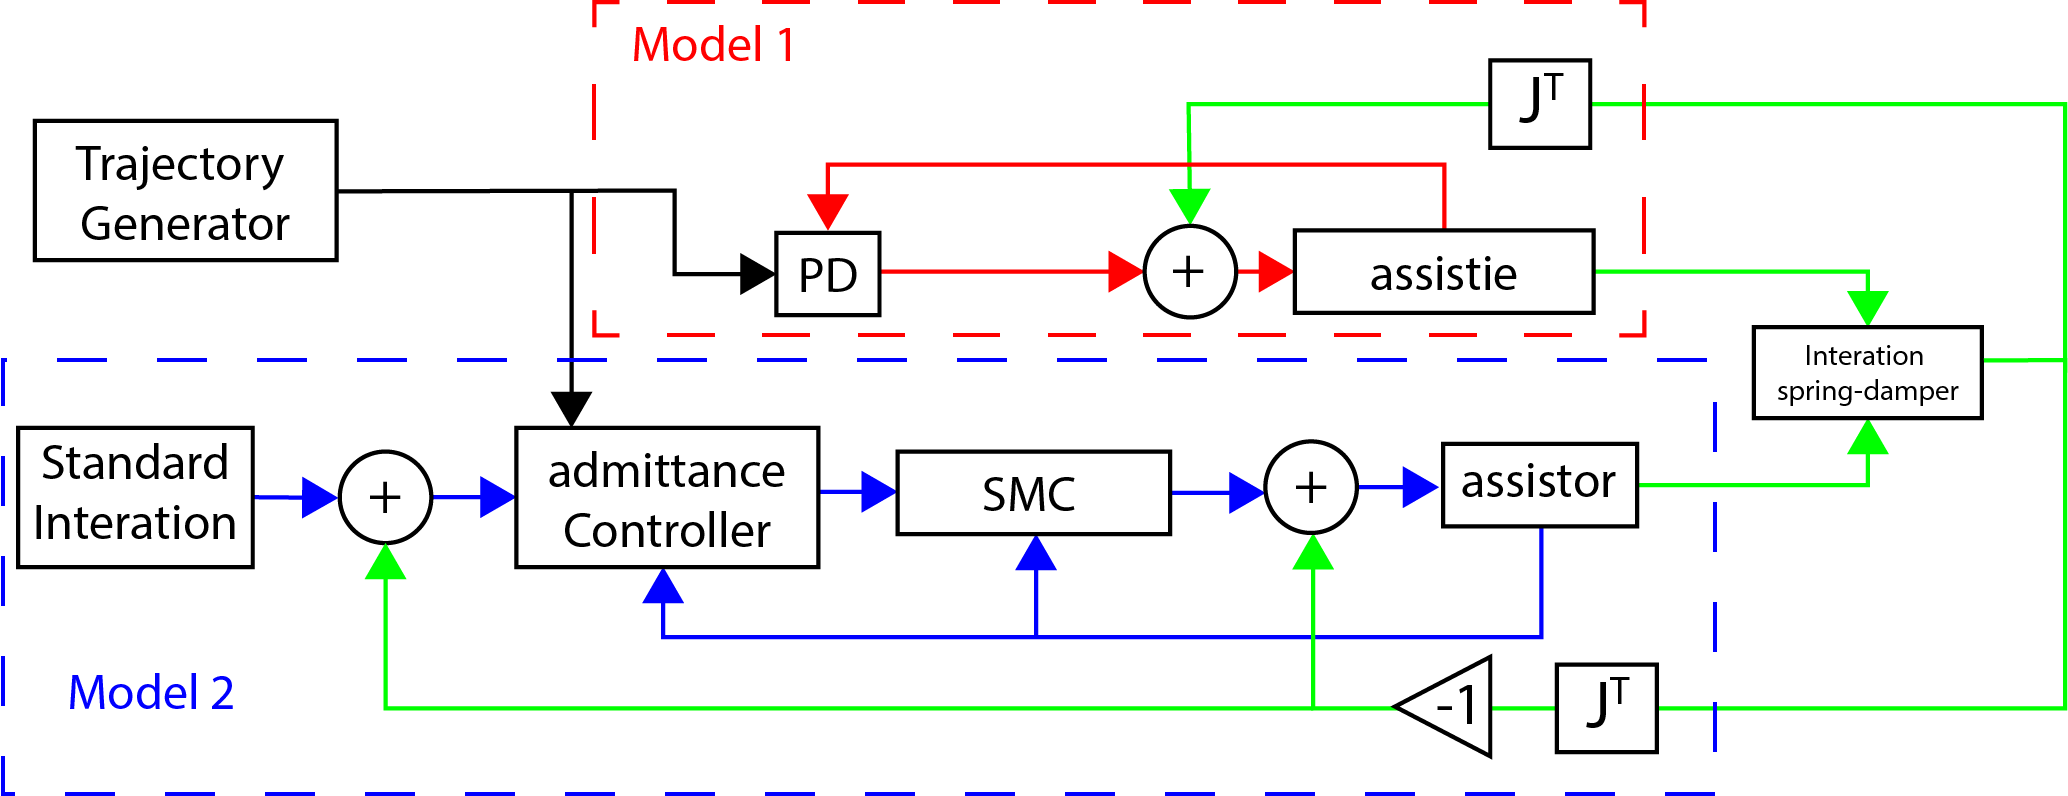
\includegraphics[scale=0.9]{images/controllers/SMC_control_diagram_overview.png}
    \caption{Control diagram for A-SMC }
    \label{fig:controlDiagram}
\end{figure*}

\autoref{eq:CooPdyn} describes the dynamics for the \textit{assistor} (abbreviated has \textit{tor}) and \textit{assistie} (abbreviated has \textit{tie}) respectively.  It should be noted that $q$ is the joint state for the respective model that they describe. The $F$ terms are the forces generated as a result of being coupled by a spring dampener described by \autoref{eq:coupling}. Additionally, $J$ is the Jacobian of each link to the connection point of the spring dampener system. Although any point on the link could be used to calculate the Jacobian matrix, the connection point is at the end of each link. This assumption does change the process, only the calculation of the Jacobian matrix. It can later be adjusted to the location of the straps of an exoskeletons.

\begin{equation} 
\begin{aligned}
    M_{tor}(q) \ddot{q} + C_{tor} (q,\dot{q}) + G_{tor}(q) &= \tau_{tor} + J_{tor}^T F \\
    M_{tie}(q) \ddot{q} + C_{tie} (q,\dot{q}) + G_{tie}(q) &= \tau_{tie} + J_{tie}^T F
\end{aligned}
    \label{eq:CooPdyn}
\end{equation}

\begin{equation}
    F = K ( \vec{x}_{tor} - \vec{x}_{tie} ) + B (\dot{ \vec{x}}_{tor} - \dot{ \vec{x}}_{tie} ) 
    \label{eq:coupling}
\end{equation}


The \textit{assisitie} system was controlled by \autoref{eq:PDcnrl}. This is simple PD control framework. $K_p$ and $K_d$ are gain matrixs and $\vec{q}_d$ is the desired position. This torque however was capped to not exceed an absolute max toque value. This was accomplished using the following method, $| \vec{\tau}_{tie}|> \vec{\tau}_{max} \rightarrow \vec{\tau}_{tie} = sign(\vec{\tau}_{tie})*\vec{\tau}_{max}$.  This did not allow the controller to generate the required torque. 

% \begin{equation}
%         \tau_{tie} = K_p( \vec{q}_d - \vec{q}_{tie} ) + K_d ( \dot{\vec{q}}_d - \dot{\vec{q}}_{tie} ) 
%     \label{eq:PDcnrl}
% \end{equation}

The admittance controls the virtual dynamics of the system and how the systems interact \cite{faulring2005haptic}. If the \textit{assastie} system is capable of following the desired motion, the \textit{assasitor} system will be less aggressive. This interaction is controlled by \autoref{eq:addmittance}, where $x_a$ is the location of the virtual system and $x_d$ is the location of the point on the pendulum link. A separate spring-dampener system is on each of the links of the system. The virtual system is defined by the following terms $M_d$, $B_d$, and $K_d$ are inertia, dampening, and stiffness, respectively. As previously stated, it is desirable to have these parameters adjust on the fly to the intention and ability of the \textit{assistie} system. The variability is controlled by \autoref{eq:intention} and \autoref{eq:varible}. Here $\alpha_{n,p}$ and $\gamma_{n,p}$ are tuning variables for the damping and stiffness of the admittance controller. The admittance will control how quickly and aggressively the \textit{assistor} system will respond. If the stiffness or dampening is too large, the model will not track the desired motion.   

\begin{equation}
    \begin{aligned}
        \tau_{int} &= M_d \ddot{e}_a + K_d e_a + B_d \dot{e}_a  \\
        e_a &= x_a - x_d 
    \end{aligned}
    \label{eq:addmittance}
\end{equation}

\begin{equation}
    \begin{aligned}
         intent &= bool ( sign(T_h) == sign(\dot{q}_d) ) \\
         \mu &= \Big|\frac{T_h}{T_{id}} \Big|
    \end{aligned}
    \label{eq:intention}
\end{equation}



\begin{equation}
    \begin{bmatrix} K_d \\ B_d \end{bmatrix} = \begin{cases}
        \begin{bmatrix} K_{p} \\ B_{p} \end{bmatrix} + \mu  \begin{bmatrix} \gamma_p  \\ \alpha_p \end{bmatrix}, intent = 1 \\
        \begin{bmatrix} K_{n} \\ B_{n} \end{bmatrix} - \mu  \begin{bmatrix} \gamma_n  \\ \alpha_n \end{bmatrix}, intent = 0
  \end{cases}
  \label{eq:varible}
\end{equation}


The A-SMC controller suffers from an abundance of tunable parameters. The admittance controller and SMC have parameters requiring synergistic tuning since these systems are connected.  A gradient descent method is used to find optimal parameters based on various cost functions and constraints for the controller.  Gradient descent is used since it should arrive quickly to a solution  \cite{piltan2012performance} \cite{wang1996course}. The goal is to minimize the objective function by updating parameters. This method will iterate until the objective function converges to a locally optimal location. The tunable parameters for this controller are the variable admittance parameters ($K_{n,p}$, $B_{n,p}$, $\alpha_{n,p}$, $\gamma_{n,p}$) and the sliding mode controller variables ($\rho$, $\Lambda$, $\beta$).  Another important variable is the limit of the torque that the \textit{assistor} system can provide, and this limitation is important since physical real systems cannot produce infinite torque. Motors and gearboxes present real limitations on the system. This method allows for the maximum torque to be used, has a hard limitation, and allows for the minimal limit to be found.


The optimization was calculated using Simulink Response Optimization\footnote{https://www.mathworks.com/help/sldo/response-optimization.html}. Several cost functions were tested to find the optimal performance, and the model was trained to follow a polynomial trajectory. Root mean squared error (RMSE) was used for the cost function shown in \autoref{eq:RMSE}, where $x$ is the observation and $\hat{x}$ is the reference, either position or velocity. The error is summed along both the trajectory and the joints to get a scalar value. If both the position and velocity RMSE is used, it is then summed.

The gain parameters $K_p$ and $K_d$ in \autoref{eq:PDcnrl} were also tuned using the same method. The controller assumed that no assistance was provided by the \textit{assistor} system. These gains were set for the \textit{assistie} controller in the closed-loop system.

\begin{equation}
    e = \sqrt{ \frac{ \sum_1^N ( \hat{x}_i - x_i )^2 }{N}  }
    \label{eq:RMSE}
\end{equation}